\documentclass[border=4pt]{standalone}
\usepackage{amsmath,amssymb}
\usepackage{tikz}
\usetikzlibrary{positioning,arrows.meta}
\begin{document}
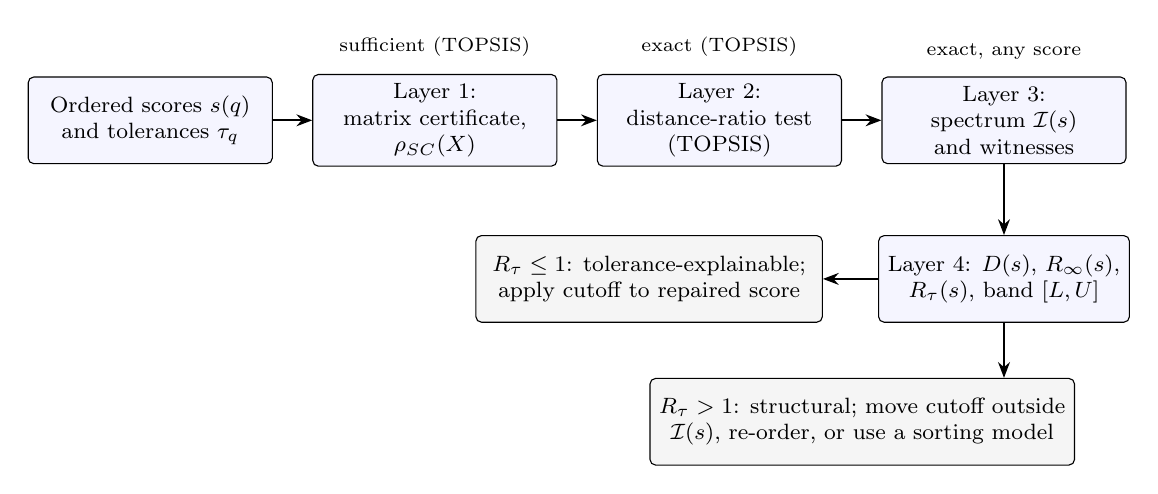
\begin{tikzpicture}[
  node distance=4mm and 5mm,
  box/.style={draw,rounded corners=2pt,align=center,font=\footnotesize,minimum height=11mm,minimum width=31mm,fill=blue!4},
  dec/.style={draw,rounded corners=2pt,align=center,font=\footnotesize,minimum height=11mm,minimum width=44mm,fill=black!4},
  arr/.style={-{Stealth[length=2mm]},thick}]
\node[box](in){Ordered scores $s(q)$\\and tolerances $\tau_q$};
\node[box,right=of in](L1){Layer 1:\\matrix certificate,\\$\rho_{SC}(X)$};
\node[box,right=of L1](L2){Layer 2:\\distance-ratio test\\(TOPSIS)};
\node[box,right=of L2](L3){Layer 3:\\spectrum $\mathcal I(s)$\\and witnesses};
\node[box,below=9mm of L3](L4){Layer 4: $D(s)$, $R_\infty(s)$,\\$R_\tau(s)$, band $[L,U]$};
\node[dec,left=7mm of L4](ok){$R_\tau\le1$: tolerance-explainable;\\apply cutoff to repaired score};
\node[dec,below=7mm of L4,xshift=-18mm](bad){$R_\tau>1$: structural; move cutoff outside\\$\mathcal I(s)$, re-order, or use a sorting model};
\draw[arr](in)--(L1);\draw[arr](L1)--(L2);\draw[arr](L2)--(L3);\draw[arr](L3)--(L4);
\draw[arr](L4)--(ok);\draw[arr](L4.south)--(L4.south|-bad.north);
\node[font=\scriptsize,above=1mm of L1]{sufficient (TOPSIS)};
\node[font=\scriptsize,above=1mm of L2]{exact (TOPSIS)};
\node[font=\scriptsize,above=1mm of L3]{exact, any score};
\end{tikzpicture}
\end{document}
